% !TeX root = ..\discrete_math.tex
\chapter{Теория графов}
\section{Основные определения}
Пусть $M$ и $N$ - два конечных множества. Будем называть пару множеств $\langle M, N \rangle$ \textbf{ориентированным графом}.
При этом элементы множества $M$ называются \textbf{вершинами} графа, элементы множества $N$ - \textbf{дугами} графа. 
Граф, у которого направления соединения не определены, называется \textbf{неориентированным графом}. В них
соединения называются \textbf{ребром}, а вершина - \textbf{узлом}.

\begin{figure*}[!h]
    \centering
    \begin{minipage}[t]{4cm}
        \centering
        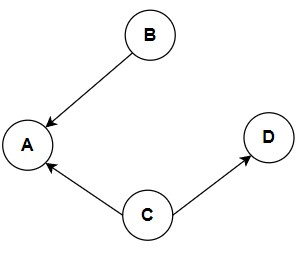
\includegraphics{graph_or.jpg}
        \caption{Ориентированный граф}
    \end{minipage}
    \hspace{3cm}
    \begin{minipage}[t]{4cm}
        \centering
        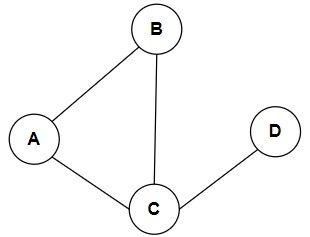
\includegraphics{graph_nor.jpg}
        \caption{Неориентированный граф}
    \end{minipage}
\end{figure*}

\textbf{Висячей вершиной} называется вершина, которая соединена только с одной соседней вершиной.

\textbf{Степенью вершины} называется количество ребер, соединенных с этой вершиной.
Если степень вершины равна 0, то такая вершина называется \textbf{изолированной}.
Степень вершины может быть \textbf{входящей} и \textbf{исходящей}. Входящая степень вершины $v$
это количество ребер вида $\langle i, v \rangle$, то есть количество ребер которые входят в $v$.
Исходящая степень вершины $v$ это количество ребер вида $\langle v, i \rangle$, то есть количество ребер
которые входят из $v$.

\begin{thm}
    В любом графе всегда найдутся хотя бы две вершины с одинаковой степенью.
\end{thm}

Дуга, у которой начало и конец совпадают, называется \textbf{петлей}.

Граф $\langle M', N'\rangle$ называется \textbf{простым путем}, если
\begin{enumerate}
    \item число его дуг $k$ на единицу меньше числа вершин
    \item можно так пронумеровать $M'$ числами от 0 до $k$ и $N'$ числами от 1 до $k$,
    что для любой дуги $u \in N'$
\end{enumerate}

Пусть $num$ - это получение номера дуги или вершины, а $beg(u)$ и $end(u)$ начало и конец дуги 
$u$ соответственно. Тогда для любой дуги $u$ в графе верно выражение:
\begin{equation}
    \label{simple_path}
    num(u) = num(end(u)) = num(beg(u)) + 1
\end{equation}
Различие между \textbf{путем} и \textbf{простым путем} заключается в том, что во втором случае
недопустимы повторы вершин и дуг в пути.
\begin{figure}[h]
    \centering 
    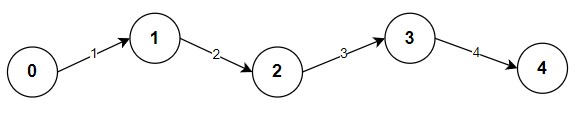
\includegraphics{simple_path.jpg}
    \caption{Простой путь}
\end{figure}

Граф $\langle M', N'\rangle$ называется \textbf{цепью}, если:
\begin{enumerate}
    \item число его дуг $k$ на единицу меньше числа вершин
    \item можно так пронумеровать $M'$ числами от 0 до $k$ и $N'$ числами от 1 до $k$,
    что для любой дуги $u \in N'$
\end{enumerate}
То есть, он включает либо условие простого пути \ref{simple_path}, либо
\begin{equation}
    \label{chain}
    num(u) = num(end(u)) + 1 = num(beg(u))
\end{equation}
Дуги, для которых выполняется \ref{simple_path}, принято называть \textbf{положительно ориентированными},
а те, для которых выполняется \ref{chain} \textbf{отрицательно ориентированными}.

\begin{figure}[h]
    \centering 
    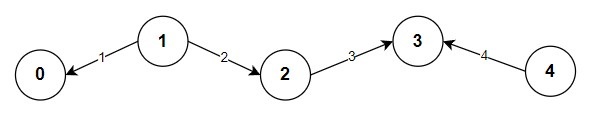
\includegraphics{chain.jpg}
    \caption{Цепь}
\end{figure}

Граф $\langle M', N'\rangle$ называется \textbf{контуром}, если
\begin{enumerate}
    \item число дуг $k$ равно числу вершин
    \item можно так пронумеровать $M'$ и $N'$ числами от 1 до k, что для любой
    дуги $u \in N'$
\end{enumerate}
\begin{equation}
    num(u) \stackrel{\text{mod k}}{=} num(end(u)) \stackrel{\text{mod k}}{=} num(beg(u)) + 1
\end{equation}
Иными словами, контур - это простой путь, где начало и конец совпадают.

\begin{figure}[h]
    \centering 
    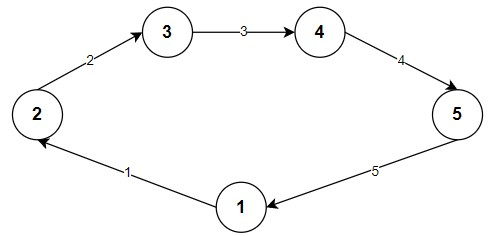
\includegraphics{loop.jpg}
    \caption{Контур}
\end{figure}

\vspace{3mm}

Граф $\langle M', N'\rangle$ называется \textbf{циклом}, если
\begin{enumerate}
    \item число дуг $k$ равно числу вершин
    \item можно так пронумеровать $M'$ и $N'$ числами от 1 до $k$, что для любой дуги $u \in N'$
\end{enumerate}
\begin{equation}
    num(u) \stackrel{\text{mod k}}{=} num(end(u)) \stackrel{\text{mod k}}{=} num(beg(u)) + 1
\end{equation}
либо
\begin{equation}
    num(u) \stackrel{\text{mod k}}{=} num(end(u)) + 1 \stackrel{\text{mod k}}{=} num(beg(u))
\end{equation}
Цикл - это цепь, в которой начало и конец совпадают.
\begin{figure}[h]
    \centering 
    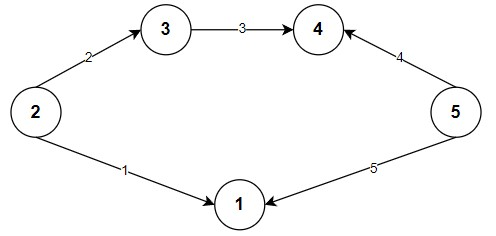
\includegraphics{cycle.jpg}
    \caption{Цикл}
\end{figure}

\section{Связность. Компоненты связности и сильной связности}
Граф $\langle M, N\rangle$ называется \textbf{связным}, если любые две различные его
вершины можно соединить цепью. Любой граф может быть однозначно разделен на максимальные
связные подграфы, которые называют его \textbf{компонентами связаности}.
\begin{figure}[h]
    \centering 
    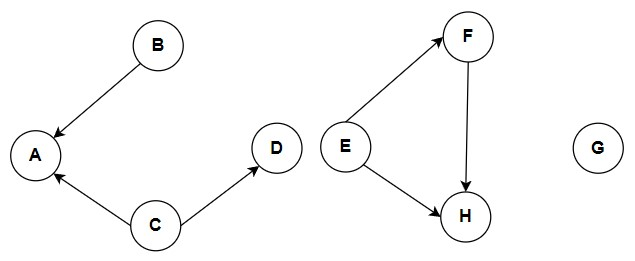
\includegraphics{connectivity.jpg}
    \caption{Пример несвязного графа}
\end{figure}

Граф $\langle M, N\rangle$ называется \textbf{сильно связным}, если любые две различные
вершины A и B можно соединить путем с началом в A и концом в B. В любом графе можно однозначно
выделить максимальные сильно связные подграфы, которые называются его \textbf{компонентами сильной связности}.
\begin{thm}
    Граф компонент сильной связности не имеет контуров.
\end{thm}

\section{Матричные представления графов}
Прежде чем приступить к понятию "дерево" , изучим различные способы представления графов.
Наиболее известные формы это \textbf{матрица инциденций} и \textbf{матрица смежности}.
Для начала рассмотрим более простой вариант - матрицу смежности.

\vspace{3mm}

\textbf{Матрицей смежности} графа $\langle M, N\rangle$ называется такая квадратная матрица $M \times M$
(то есть индексами строк и столбцов являются вершины графа), 
в которой значением пересечения $i$-ой строки и $j$-го столбца является число дуг с началом в $i$ и концом $j$.

\begin{figure}[!h]
    \centering 
    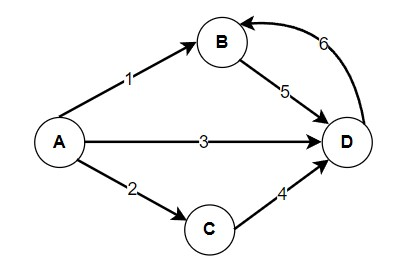
\includegraphics{graph_1.jpg}
    \caption{Граф}
    \label{graph_for_matrix}
\end{figure}

\begin{figure*}[!h]
    \centering
    \begin{minipage}[t]{4cm}
        \centering
        \begin{tabular}[c]{ | l | l | l | l | l | l | l | l |}
            \hline
              & 1  & 2  & 3  & 4  & 5  & 6  \\ \hline
            A & 1  & 1  & 1  & 0  & 0  & 0  \\ \hline
            B & -1 & 0  & 0  & 0  & 1  & -1 \\ \hline
            C & 0  & -1 & 0  & 1  & 0  & 0  \\ \hline
            D & 0  & 0  & -1 & -1 & -1 & 1  \\
            \hline
        \end{tabular}
    \end{minipage}
    \hspace{3cm}
    \begin{minipage}[t]{4cm}\
        \centering
        \begin{tabular}[c]{ | l | l | l | l | l |}
            \hline
              & A & B & C & D \\ \hline
            A & 0 & 1 & 1 & 1 \\ \hline
            B & 0 & 0 & 0 & 1 \\ \hline
            C & 0 & 0 & 0 & 1 \\ \hline
            D & 0 & 1 & 0 & 0 \\
            \hline
        \end{tabular}
    \end{minipage}
    \caption{Способы матричного представления графа \ref{graph_for_matrix}: матрица инциденций
    и матрица смежности соответственно}
\end{figure*}

\hspace{3mm}

\textbf{Матрицей инциденции} графа $\langle M, N\rangle$ называется такая матрица $M \times N$, 
где индексами строк являются вершины, а индексами столбцов дуги. Элемент на пересечении $i$-ой строки и $j$-ого
столбца равен 1, если является началом в вершине под $i$-ым индексом и принадлежит дуге под $j$-ым индексом. Если же данная
дуга имеет конец в этой вершине, то ставится -1.

\section{Деревья}
Чтобы ввести термин "дерево", нам нужно изучить следующую теорму:
\begin{thm}
    В связном графе $\langle M, N \rangle$ найдется частичный граф связный граф
    $\langle M, N' \rangle$, в котором количество вершин больше количества дуг на единицу. Пусть $|N'| = k$, 
    тогда если пронумеровать вершины из M числами от 0 до k, а дуги из N' числами от 1 до k
    таким образом, что для любой дуги $u \in N'$ выполняется соотношение
    \begin{equation}
        num(u) = max\{num(beg(u)), num(end(u))\}
    \end{equation}
\end{thm}
\begin{sle}
    Если $|N| < |M| - 1$, граф не может быть связан.
\end{sle}
\begin{sle}
    Если $|N| > |M| - 1$, граф содержит циклы.
\end{sle}

Связный граф, в котором число дуг на 1 меньше числа вершин, называется
\textbf{деревом}. Такие деревья могут не иметь корня, в отличие от тех деревьев,
которые мы обычно представляем. Если подобное дерево имеет корень, то оно называется 
\textbf{ориентированным деревом}.
Дерево, являющееся частичным графом связного графа, называется его \textbf{остовным деревом} (spanning tree).

Теперь можно присутпить к изучению алгоритма нахождения остовного дерева методом вычеркивания.

\hspace{5mm}

\textbf{Алгоритм нахождения остовного дерева}
\begin{enumerate}
    \item В матрице инцидентности $N \times N-1$ проверяем наличие нулевых строк. 
    Если есть, то имеем неостовное дерево.
    \item Если нет, то проверяем наличие строк с одной единицей
    и вычеркиваем строку и столбец, проходящие через эту единицу
    \item Повторяем пункт 1 и 2 до тех пор, пока не придем к выводу, что это неостовное дерево или
    если все столбцы вычеркнуты, то рассмотренные ребра образуют остовное дерево
\end{enumerate}

Рассмотрим пример. Имеем следующую матрицу инцидентности:
\begin{table}[h]
    \centering
    \begin{tabular}[c]{ | l | l | l | l | l | l | l | l | l | l | }
        \hline
        1 & 2 & 3 & 4 & 5 & 6 & 7 & 8 & 9 & 10 \\ \hline
        1 & 0 & 0 & 1 & 0 & 1 & 0 & 0 & 0 & 0 \\ \hline
        0 & 1 & 0 & 0 & 0 & 0 & 0 & 0 & 1 & 1 \\ \hline
        1 & 1 & 1 & 0 & 0 & 0 & 0 & 0 & 0 & 0 \\ \hline
        0 & 0 & 0 & 0 & 0 & 1 & 1 & 1 & 0 & 0 \\ \hline
        0 & 0 & 1 & 0 & 0 & 1 & 1 & 0 & 0 & 0 \\ \hline
        0 & 0 & 0 & 1 & 1 & 0 & 0 & 0 & 0 & 0 \\ 
        \hline
    \end{tabular}
    \caption{Матрица инциденций}
\end{table}

Теперь проверим, являются ли ребра 1, 2, 5, 7 и 8 остовным деревом:
\begin{figure}[!h]
    \centering 
    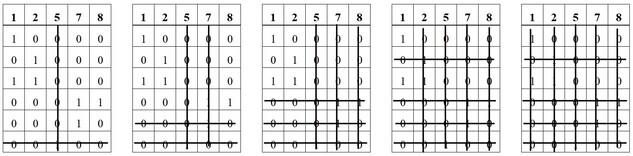
\includegraphics{matrix1.jpg}
\end{figure}

Так как в процессе у нас не возникло нулевых строк и в итоге все строки и столбцы 
были зачеркнуты, данные ребра образуют остовное дерево.
Например, ребра 1, 2, 4, 5 и 8 не будут образовывать остовное дерево, так как 5
строчка будет состоять только из нулей.

\section{Задача о кратчайшем пути}
Для начала введем новый термин "весовая матрица". Пусть у нас есть ориентированный граф,
дуги которого имеют определенный вес (положительное число). 

\textbf{Весовая матрица} это квадратная матрица $M \times M$
(индексами строк и столбцов являются вершины), где элемент под $i$-ой строкой и $j$-ым столбцом имеет вес дуги из вершины
под индексом $i$ в вершину под индексом $j$.
\begin{figure}[!h]
    \centering 
    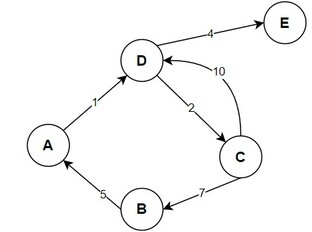
\includegraphics{weight_graph_1.jpg}
    \caption{Граф}
    \label{weight_graph}
\end{figure}

\begin{table}[h]
    \centering
    \begin{tabular}[c]{ | l | l | l | l | l | l | }
        \hline
          & A & B & C & D & E \\ \hline
        A & 0 & $\infty$ & $\infty$ & 1 & $\infty$ \\ \hline
        B & 5 & 0 & $\infty$ & $\infty$ & $\infty$ \\ \hline
        C & $\infty$ & 7 & 0 & 10 & $\infty$ \\ \hline
        D & $\infty$ & $\infty$ & 2 & 0 & 4 \\ \hline
        E & $\infty$ & $\infty$ & $\infty$ & $\infty$ & 0 \\
        \hline
    \end{tabular}
    \caption{Весовая матрица графа \ref{weight_graph}}
\end{table}
Чтобы не путаться и обозначить, что из $i$-ой вершины в $j$-ую нет пути, будем писать знак 
бесконечности.

Теперь, собственно, приступим к самой задаче нахождения кратчайшего расстояния между двумя вершинами.
Предположим, нам нужно найти кратчайший путь из A в F для матрицы \ref{weight_matrix}:
\begin{table}[h]
    \centering
    \begin{tabular}[c]{ | l | l | l | l | l | l | l | }
        \hline
          & A & B & C & D & E & F \\ \hline
        A & 0 & 10 & 3 & $\infty$ & $\infty$ & $\infty$ \\ \hline
        B & $\infty$ & 0 & 5 & $\infty$ & $\infty$ & 3 \\ \hline
        C & $\infty$ & 4 & 0 & 2 & 6 & $\infty$ \\ \hline
        D & $\infty$ & 1 & $\infty$ & 0 & 5 & $\infty$ \\ \hline
        E & $\infty$ & $\infty$ & $\infty$ & $\infty$ & 0 & 4 \\ \hline
        F & $\infty$ & $\infty$ & $\infty$ & $\infty$ & $\infty$ & 0 \\
        \hline
    \end{tabular}
    \caption{Весовая матрица}
    \label{weight_matrix}
\end{table}

Создадим новую таблицу, в которой за строки возьмем количество дуг, которые
можно провести из одной вершины в другую, а за столбцы сами эти вершины. Будем построчно
заполнять таблицу, тем самым найдя кратчайший путь из A в F.

\begin{table}[h]
    \centering
    \begin{tabular}[c]{ | l | l | l | l | l | l | l | }
        \hline
          & A(1) & B(2) & C(3) & D(4) & E(5) & F(6) \\ \hline
        1 & 0 & 10(1) & 3(1) & $\infty$ & $\infty$ & $\infty$ \\ \hline
        2 & 0 & 7(3) & 3(1) & 5(3) & 9(3) & 13(2) \\ \hline
        3 & 0 & 6(4) & 3(1) & 5(3) & 9(3) & 10(2) \\ \hline
        4 & 0 & 6(4) & 3(1) & 5(3) & 9(3) & 9(2) \\ \hline
        5 & 0 & 6(4) & 3(1) & 5(3) & 9(3) & 9(2) \\ \hline
        6 & 0 & 6(4) & 3(1) & 5(3) & 9(3) & 9(2) \\
        \hline
    \end{tabular}
    \caption{Поиск кратчайшего пути из A в F}
    \label{short_s}
\end{table}

Логика такая: смотрим, как можно попасть в данную вершину с помощью весовой матрицы.
Далее если есть смотрим на строчку выше в \ref{short_s} и ищем способы попасть в вершину за k дуг. Прокомментирую 
первые 2 строчки:
\begin{enumerate}
    \item Так как мы начинаем с вершины A, то ставим 0. Далее смотрим, как можно попасть 
    в вершину B за 1 дугу по весовой матрице. Смотрим на столбец B: так как мы начинаем путь из вершины A
    и до других вершин не дошли, самый оптимальный путь это попасть в B из A за 10. В скобочках пишем из 
    какой вершины попали. С остальными вершинами такая же логика. Если попасть в вершину за k дуг пока нельзя, ставим $\infty$
    \item С А ничего не меняется, смотрим на B. В весовой матрице можно заметить, что в B можно попасть из
    A, C, D. Из А за 10, из C за 4 и из D за 1. Смотрим на предыдущую строчку и ищем эти вершины. За одну дугу в B из A
    мы попали за 10. В C мы можем попасть из A за 3, а в D пока не можем. И так вариант A -> C -> B выгоднее, чем A -> B, 
    то записываем 4 + 3 = 7(3). Так как в C выгоднее всего попасть из A, то так и оставляем. В D мы можем попасть из C, то есть
    A -> C -> D (3 + 2 = 5). В E из С и D, но так как в D, судя по предыдущей строчке, мы попасть никак не можем за 1 дугу,
    выбираем путь из С, то есть A -> C -> E (3 + 6 = 9). В F мы можем попасть из B и E. По предыдущей строчке смотрим,
    что в E мы пока попасть не можем, а вот в B из A можем. Значит, путь получается следующим: A -> B -> F (10 + 3 = 13)
    \item По такой же логике заполняем остальные строчки.
\end{enumerate}
В результате смотрим на последнюю строчку и столбец F. У нас получилось 9(2). Чтобы восстановить путь, поднимаемся по строчкам
и смотрим на вершину в скобках. Как результат: A -> C -> D -> B -> F